% !TEX root = Modi_RobustCode.tex
\chapter{여러 가지 곡면}


함수의 연속성이나 미분가능성은 각각의 점에서 정의하기 때문에 \myem{국소적 개념}이라고 말한다. 
하지만 이를 이용하여 주어진 함수의 정의역 전체에서 연속성이나 미분가능성을 정의하므로 함수의 대역적 성질에 대해서도 이야기 할 수 있다. 같은 이유에 의해 가우스곡률과 평균곡률도 국소적 개념이라고 할 수 있지만 이러한 기하학적 개념이 곡면의 국소적 성질이나 모양에만 영향을 미치는 것만은 아니다. 
예를 들어, 주어진 곡면의 모든 점에서 가우스곡률이 $0$이면 이 곡면은 평면이 된다. \myem{가우스곡률}이 모든 점에서 $0$이 아닌 상수이면 이 곡면은 구면 또는 구면의 일부가 된다. 이 장에서는 4장에서 배운 내용을 기초로 곡면의 대역적(global)
성질을 살펴보고 여러가지 곡면의 예를 통하여 한 단계 더 심화된
곡면이론에 대하여 알아본다. 1절에서는 곡면의 대역적 성질에 관한 몇 가지 정리를 소개하고 2절에서는 곡면이론에서 매우 중요한 역할을 하는 \myem[surface of revolution]{회전면}에 대하여 다룬다. \myem{회전면}은 한 곡선을 고정된 한 축을 중심으로 회전시켰을 때 얻어지는
곡면으로 가우스곡률을 비교적 쉽게 구할 수 있다. 또한, 어떤 함수가 주어졌을 때 그 함수를 가우스곡률로 갖는 곡면의
존재성에 관한 문제를 해결해 줄 수 있는 곡면이기도 하다.
3절에서는 곡면의 또다른 예인 \myem[ruled surface]{선직면}에 대하여 알아본다. 선직면은 한 곡선과 그 곡선 위에 정의된
벡터장에 의해 만들어지는 곡면으로 가우스곡률이 항상 $0$보다 작거나 같다. 끝으로 4절에서는
\myem[minimal surfaces]{극소곡면}에 대하여 알아보기로 한다. 극소곡면은 국소적으로 경계를 고정했을 때 넓이가 최소가 되는 곡면이라고 말할 수 있다.



\section{대역적 곡면이론}

이 절에서는 \myem{대역적(global) 곡면이론}에 관한 몇 가지 정리를
소개하고자 한다.
여기서는 주로 \myem{가우스곡률}이 곡면의 위상구조에 어떤 영향을
미치는지에 대하여 알아보기로 한다.  지금까지 그래 왔듯이
앞으로도 \myem{정칙곡면} $M$은 항상 연결집합이라는 것을 가정한다.

\begin{thm}[배꼽점]\label{thm511}
$M \subset \mathbf{R}^3$을 가향 정칙곡면이라 할 때,
가우스함수 $Z$의 미분이 $0$이면, 즉 $\mathrm{d}Z = 0$이면 $M$은 평면
또는 평면의 일부분이다.
\end{thm}

\begin{proof}
한 점 $ \mathbf{p} \in M$을 고정하자. $\mathrm{d}Z = 0$이라는 것은
가우스함수 $Z$가 상수함수임을 나타낸다. 따라서 $M$이
$ \mathbf{p}$를 지나고 $Z$에 수직인 평면에 포함되는 것을
 보이면 된다. $ \mathbf{q}\in M$를 임의의 점이라 하면,
$M$은 연결집합이므로 곡선 $\alpha :[0,1] \to M$이 존재하여
$\alpha(0) =  \mathbf{p}, \alpha(1) =  \mathbf{q}$이다.
이제 함수 $h$를
\[
h(t) = \langle \alpha(t) -  \mathbf{p}, Z \rangle
\]
라 정의하면, $h(0)  =  0$이고 함수 $h$를 $t \in (0,1)$에 대하여 미분하면
\[
h'(t) = \langle \alpha'(t), Z \rangle = 0.
\]
따라서 $h$는 \myem{열린구간} $(0,1)$에서 상수함수이고 $[0,1]$에서 연속함수이므로
닫힌구간 $[0,1]$에서 상수함수이다. $h(0) = 0$이므로 $h(t) = 0$.
특히 $h(1) = \langle  \mathbf{q}-
 \mathbf{p}, Z\rangle = 0$이다. 그러므로 임의의 점
 $ \mathbf{q}\in M$는 우리가 원하는 평면에 놓인다.
\end{proof}

정의에 의해 점 $ \mathbf{p}\in M$가 평면점이면
$\kappa_1( \mathbf{p}) = \kappa_2( \mathbf{p}) = 0$이다. 그리고
이것은 $\mathrm{d}Z_{ \mathbf{p}} = 0$인 것과 동치이다.
정리 \ref{thm511}은 정칙곡면 $M$의 모든 점이 평면점이면 $M$은 평면이라는 것을
보여준다.

\myem{법곡률}의 최대값과 최소값이 일치하는 점을 \myem{배꼽점}이라 말한다. 예를 들어
평면이나 구면의 모든 점은 \myem{배꼽점}이다 (4장1절 참고).
중요한 것은 그것의 역 또한 성립한다는 사실이다.

\begin{thm}\label{thm512}
$M \subset \mathbf{R}^3$을 연결 정칙곡면이라 하자. 만일 $M$의
모든 점이 배꼽점이면 $M$은 구면이나 평면, 또는 그것의 일부분이다.
\end{thm}

\begin{proof}
\textbf{첫째단계:} 점 $\mathbf{p} \in M$가 배꼽점이면 모든 접벡터
$\mathbf{v}\in T_{\mathbf{p}}$는 \myem{주곡률 방향}임을 보이자.

$\mathbf{p}\in M$에서
$\kappa_1(\mathbf{p}) = \kappa_2(\mathbf{p}) = k$이고 $\mathbf{e}_1, \mathbf{e}_2$를
주곡률 방향이라고 하자. 그러면 임의의 접벡터 $\mathbf{v} = a \mathbf{e}_1 +
b \mathbf{e}_2 \in T_{\mathbf{p}} M$에 대하여
\begin{align}
\mathrm{d}Z_{\mathbf{p}}(\mathbf{v})
&= a\, \mathrm{d}Z_{\mathbf{p}}(\mathbf{e}_1) +
b \,\mathrm{d}Z_{\mathbf{p}}(\mathbf{e}_2)\\
&= -a \,k\,  \mathbf{e}_1 - b\, k\,\mathbf{e}_2\\
&= -k \,\mathbf{v}.
\end{align}

\textbf{둘째단계:} $\mathbf{x}: D \subset \mathbf{R}^2 \to M$을 좌표함수라 하고 $V = \mathbf{x}(D)$라
놓자. 그러면 $V$는 평면 또는 구면의 일부분임을 증명하자.

가정에 의해 각 점 $\mathbf{q}\in V$가 배꼽점이므로 \textbf{첫단계}에 의해
임의의 접벡터 $\mathbf{v} = a \mathbf{x}_u + b \mathbf{x}_v \in
T_{\mathbf{q}} M$에 대하여
\begin{equation}
\mathrm{d}Z_{\mathbf{q}}(\mathbf{v}) = \lambda(\mathbf{q}) \mathbf{v}.
\label{eqn21010}
\end{equation}
여기서 $\lambda(\mathbf{q}) = - \kappa_1(\mathbf{q}) = -\kappa_2(\mathbf{q})$는 $V$에서
정의된 미분가능한 함수이다.

\begin{itemize}
\item[\textbf{(i)}] $\lambda$는 \myem{상수함수}이다.
식 \eqref{eqn21010}\를 풀어쓰고 도움정리를 이용하면
\begin{align}
&a dZ(\mathbf{x}_u) + b dZ(\mathbf{x}_v) = \lambda (a \mathbf{x}_u + b \mathbf{x}_v)\\
\Leftrightarrow{}& a Z_u + b Z_v = \lambda (a \mathbf{x}_u + b \mathbf{x}_v).
\end{align}
$\mathbf{v}$는 임의의 \myem{접벡터}이므로
\[
Z_u = \lambda \mathbf{x}_u, \qquad Z_v = \lambda \mathbf{x}_v.
\]
첫째 식을 $v$에 대하여 미분하고 둘째 식을 $u$에 대하여 미분하면
\begin{align}
Z_{uv} &= \lambda_v \mathbf{x}_u + \lambda  \mathbf{x}_{uv}\\
Z_{v u} &= \lambda_u \mathbf{x}_v + \lambda  \mathbf{x}_{vu}.
\end{align}
이 두 식의 뺄셈을 하면
\[
\lambda_v \mathbf{x}_u - \lambda_u  \mathbf{x}_v =0
\]
을 얻는다. $\mathbf{x}_u$와 $\mathbf{x}_v$는 각각의 접평면에서
일차독립이므로 각 점 $\mathbf{q}\in V$에 대하여
\[
\lambda_u = \lambda_v = 0
\]
을 만족한다. $V$연결집합이므로 다변수해석학의 이론에 의해
$\lambda$는 집합 $V$위에서 상수함수이다.

\item[\textbf{(ii)}] $\lambda  = 0$이면 $V$는 평면의 일부이다.

이 경우 $\mathrm{d}Z = 0$이므로 정리 \ref{thm511}에 의해 $V$는 평면 또는 평면의
일부이다.

\item[\textbf{(iii)}] $\lambda \ne 0$이면 $V$는 구면의 일부이다.

다음 벡터방정식
\begin{equation}
\mathbf{y}(u, v) = \mathbf{x}(u, v) - \frac{1}{\lambda} Z(u, v)\label{eqn21011}
\end{equation}
을 생각하자.
\begin{align}
\mathbf{y}_u &= \mathbf{x}_u - \frac{1}{\lambda} Z_u
= \mathbf{x}_u - \frac{1}{\lambda} \mathrm{d}Z(\mathbf{x}_u)\\
&= \mathbf{x}_u - \frac{1}{\lambda}\left(\lambda \mathbf{x}_u \right) =0.
\end{align}
같은 방법으로
\[
\mathbf{y}_v = 0
\]
임을 보일 수 있다. 따라서 $\mathbf{y} = \mathbf{y}_0$는 상수벡터이다.
그러므로 식 \eqref{eqn21011}에서
\[
\Vert  \mathbf{x} - \mathbf{y}\Vert^2 = \frac{1}{\lambda^2} = \text{상수}
\]
즉, $V = \mathbf{x}(D)$는 반지름이 $\displaystyle{\frac{1}{|\lambda|}}$인
구면의 일부분이다.
\end{itemize}


\begin{figure}
\centering{%
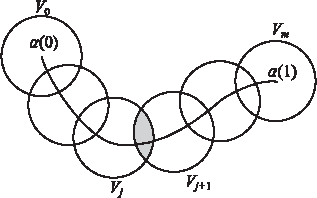
\includegraphics{5-01}
}
\caption{멋진 그림}\label{fig:wonderful_figure}
\end{figure}


\textbf{셋째단계:} $M$ 전체가 평면이나 구면 또는 그것의 일부분임을 증명하자.

둘째 단계에서 좌표함수로 나타낼 수 있는 영역에 대하여 정리가 성립하는 것을
보였다. 셋째 단계에서는 국소적 성질을 대역적 성질로 확장시키는 방법을 이용하여
곡면 전체에 대하여 정리가 성립함을 보이자.

한 점 $\mathbf{p}\in M$을 고정하고 $V\subset M$을
$\mathbf{p}$의 근방으로 하나의 좌표함수로 나태낼 수 있는 영역이라고 하자.
$\mathbf{q}\in M$를 $\mathbf{q}\ne \mathbf{p}$인 임의의 점이라고 하면
연결집합의 정의에 의해
$\alpha(0) = \mathbf{p}$이고 $\alpha(1) = \mathbf{q}$를 만족하는
연속인 곡선 $\alpha : [0,1] \to M$이 존재한다. 각각의 $\alpha(t)$에 대하여
$V_t \subset M$를 하나의 좌표함수로 나타낼 수 있는 $\alpha(t)$의 근방을 택하자.
그러면
\[
\bigcup_{t \in [0,1]}\alpha^{-1}(V_t)
\]
는 닫힌구간 $[0,1]$의 \myem[open covering]{열린덮개}가 된다. $[0,1]$이 \myem{옹골집합}이므로
유한개의 \myem{열린덮개} $\alpha^{-1}(V_1)$, $\cdots$, $\alpha^{-1}(V_m)$, $V_1 = V$가 존재하여
\[
\bigcup_{j= 1}^m\alpha^{-1}(V_j) = [0,1]
\]
이고, 각 $j=1, \cdots, m$에 대하여
\begin{equation}
\alpha^{-1}(V_j) \cap \alpha^{-1}(V_{j+1})\ne \emptyset\label{eqn21012}
\end{equation}
%\vspace{1.5in}
를 만족한다(\figurename~\ref{fig:wonderful_figure}). 따라서
\[
\alpha([0,1]) \subset \bigcup_{j=1}^m V_j.
\]

둘째 단계에 의해 $V_1 = V$는 평면의 일부이거나 구면의 일부이다. 만일 $V_1 = V$가 평면의 일부이면 식 \eqref{eqn21012}에 의해
모든 $j = 1, \cdots, m$에 대하여 $V_j$는 \textbf{같은} 평면의 일부이어야 한다.
따라서 점 $\mathrm{q}$의 근방인 $V_m$도 같은 평면의 일부이다.
만일 $V_1$이 구면의 일부이면 같은 이유에 의해 모든 $j$에 대하여
$V_j$도 같은 구면의 일부이어야만 한다. 결과적으로 $M$ 전체는
평면이거나 구면 또는 그것의 일부분이다.
\end{proof}


정리 \ref{thm512}에 의하면 연결집합인 정칙곡면
 $M$의 모든 점이 배꼽점이면 $M$은 구면 또는 평면이 된다. 따라서
다음 정리가 성립한다.

\begin{cor}\label{cor513}
정칙곡면 $M$의 모든 점이 배꼽점이면 $M$은 상수인 가우스곡률
$K \ge 0$을 갖는다.
\end{cor}

\begin{thm}[정칙곡면과 구의 관계]\label{thm514}
\myem{정칙곡면} $M \subset  \mathbf{R}^3$의 모든 점이 배꼽점이고
$K > 0$이면 $M$은 반지름이 $\displaystyle \frac{1}{\sqrt K}$인 구면 또는
구면의 일부분이다.
\end{thm}

\begin{cor}[당연한 따름정리]\label{surface}
정칙곡면 $M \subset  \mathbf{R}^3$의 모든 점이 \myem{배꼽점}이고
$K > 0$이면 $M$은 반지름이 $\displaystyle \frac{1}{\sqrt K}$인 구면 또는
구면의 일부분이다.
\end{cor}

\begin{proof}[날쌘 정리의 증명]
이 정리는 정리 \ref{thm512}와 따름정리 \ref{cor513}에 의하여 성립한다.
또한 다음과 같은 방법으로 직접 보일 수도  있다.

가정에 의해 각 점 $\mathbf{p}\in M$에서
$\kappa_1(\mathbf{p}) = \kappa_2( \mathbf{p}) = k(\mathbf{p}) \ne 0$이므로
$\kappa(\mathbf{p}) > 0$을 가정해도 된다.
한 점 $\mathbf{p} \in M$을 고정하고 점 $\mathbf{c}$를
\[
\mathbf{c} = \mathbf{p} + \frac{1}{k(\mathbf{p})}
Z(\mathbf{p})
\]
라 놓자. 곡면 위의 임의의 점 $\mathbf{q}\in M$에 대하여 $M$이
연결집합이므로
$\alpha(0) = \mathbf{p}$, $\alpha(1) = \mathbf{q}$인 곡선
$\alpha : [0, 1] \to M$이 존재한다. 이제 곡선 $\gamma$를
\[
\gamma(t) = \alpha(t) + \frac{1}{k(\alpha(t))} Z(\alpha(t)) =
\alpha(t) + \frac 1k Z(t)
\]
라 정의하자. 그러면 도움정리 \ref{cor513}에 의해 $K = k^2$이
상수이므로,
\[
\gamma'(t) = \alpha'(t) + \frac 1k Z'(t)
\]
이다. 한편, $M$의 모든 점이 배꼽점이므로 모든 방향이
주곡률방향이 된다. 따라서
\[
Z'(t) = dZ(\alpha'(t)) = -k \alpha'(t).
\]
그러므로 $\displaystyle \gamma'(t) = \alpha'(t) +
\frac 1k (-k \alpha'(t)) = 0.$
결과적으로
$\gamma$는 상수곡선이 되고, 따라서
\[
\mathbf{c} = \gamma(0) = \gamma(1) = \mathbf{q} +
\frac 1k Z(\mathbf{q}).
\]
다시 말해서, $\displaystyle \Vert \mathbf{q} - \mathbf{c}\Vert = \frac 1k =
\frac{1}{\sqrt K}$이다.
\end{proof}

\begin{proof}
이 정리는 따름정리 \ref{surface}에 의하여 성립한다. 한편, $M$의 모든 점이 배꼽점이므로 모든 방향이
\myem{주곡률 방향}이 된다. 따라서
\[
Z'(t) = dZ(\alpha'(t)) = -k \alpha'(t).
\]
그러므로 $\displaystyle \gamma'(t) = \alpha'(t) +
\frac 1k (-k \alpha'(t)) = 0.$
결과적으로
$\gamma$는 \myem{상수곡선}이 되고, 따라서
\[
\mathbf{c} = \gamma(0) = \gamma(1) = \mathbf{q} +
\frac 1k Z(\mathbf{q}).
\]
\end{proof}

\begin{proof}
$M$의 모든 점이 배꼽점이므로 모든 방향이
\myem{주곡률 방향}이 된다. 따라서
\[
Z'(t) = dZ(\alpha'(t)) = -k \alpha'(t).
\]
그러므로 $\displaystyle \gamma'(t) = \alpha'(t) +
\frac 1k (-k \alpha'(t)) = 0.$
결과적으로
$\gamma$는 \myem{상수곡선}이 되고, 따라서
\[
\mathbf{c} = \gamma(0) = \gamma(1) = \mathbf{q} +
\frac 1k Z(\mathbf{q}).\qedhere
\]
\end{proof}
